\documentclass[10pt]{scrartcl}

\usepackage[utf8]{inputenc}
\usepackage{tabularx}
\usepackage[ngerman]{babel}
\usepackage[automark]{scrpage2}
\usepackage{amsmath,amssymb,amstext}
%\usepackage{mathtools}
\usepackage[]{color}
\usepackage[]{enumerate}
\usepackage{graphicx}
\usepackage{lastpage}
\usepackage[perpage,para,symbol*]{footmisc}
\usepackage{listings} 
%\usepackage[pdfborder={0 0 0},colorlinks=false]{hyperref}
\usepackage{natbib}     % Neuimplementierung des \cite-Kommandos
\usepackage{bibgerm}      % Deutsche Bezeichnungen
\usepackage{color}
\usepackage{colortbl}
\usepackage{listings}
\usepackage{a4wide}
\usepackage{xspace}
\usepackage{listings}
\usepackage{epstopdf}
\usepackage{amsmath}
\usepackage[colorinlistoftodos,textsize=small,textwidth=2cm,shadow,bordercolor=black,backgroundcolor={red!100!green!33},linecolor=black]{todonotes}%disable
\usepackage{nameref}
\usepackage{titleref}
 
\usepackage[colorlinks,
	pdftex,	
	bookmarks,
	bookmarksopen=false,
	bookmarksnumbered,
	citecolor=blue,
	linkcolor=black, %orig: blue
	urlcolor=blue,
	filecolor=blue,
	linktocpage,
    pdfstartview=Fit,                                  % startet mit Ganzseitenanzeige    
	pdfauthor={Pahl, Roetting, Jaeger, Steenbuck, Muenchow, Noetzel, Steudte}]{hyperref}
    


\usepackage[all]{hypcap}
\hypersetup{pdfsubject={TT2 Problemstellung 3 : Ausarbeitung}, pdftitle={Reinforcement Learning}, pdfkeywords={Framework, Monte Carlo Methode, Dynamic Programming, Temporal Difference Learning, Reinforcement Learning}}



\lstset{numbers=left, numberstyle=\tiny, numbersep=5pt, breaklines=true, showstringspaces=false} 

%changehere
\def\titletext{TT2 Problemstellung 3 : Ausarbeitung}
\def\titletextshort{Problemstellung 3}
\author{Pascal Jäger, Stefan Münchow, Armin Steudte,\\ Milena Rötting, Sven-Andjes Pahl, Carsten Noetzel, Oliver Steenbuck}

\title{\titletext}

%changehere Datum der Übung
\date{01.06.2012}

\pagestyle{scrheadings}
%changehere
\ihead{TT2, Neitzke}
\ifoot{Generiert am:\\ \today}

\cfoot{Pascal Jäger, Stefan Münchow,\\ Armin Steudte, Milena Rötting,\\ Sven-Andjes Pahl, Carsten Noetzel, Oliver Steenbuck}


\ohead[]{\titletextshort}
\ofoot[]{{\thepage} / \pageref{LastPage}}

\setlength{\parindent}{0.0in}
\setlength{\parskip}{0.1in}

\begin{document}
\maketitle

\setcounter{tocdepth}{3}
\tableofcontents
\listoffigures
%\lstlistoflistings

\section{Fragestellung 1: V-Werte / Q-Werte}

\section{Fragestellung 2: SARSA / Q-Learning bei kleinem $\epsilon$}
\subsection{On-Policy: SARSA}
Basis für den SARSA-Algorithmus sind die Q-Werte, also Zustands-Aktions-Paare $Q(s,a)$. Die Bewertung eines solchen Zustands-Aktions-Paares erfolgt durch die unten genannte Gleichung welche auch in Abbildung \ref{fig:Sarsa} zu finden ist.\\
Der erwartete Wert $Q(s,a)$ für eine Aktion $a$ im Zustand $s$ wird dabei aktualisiert durch, den bereits ermittelten, erwarteten Wert $Q(s,a)$ und dem Schrittfaktor $\alpha$, der mit der Summe aus Reward für den Folgezustand $r_{t+1}$ und der Differenz aus dem discounted Reward für das Folge-Zustands-Aktions-Paar $\gamma Q(s_{t+1}, a_{t+1})$ und dem erwarteten Wert $Q(s,a)$ addiert wird.\\

\begin{equation}
Q(s_{t},a_{t}) \leftarrow Q(s_{t},a_{t}) + \alpha [r_{t+1} + \gamma Q(s_{t+1},a_{t+1}) - Q(s_{t},a_{t})]
\end{equation}

In Abbildung \ref{fig:Sarsa} ist zu erkennen, dass die Aktionen $a'$ im Zustand $s'$ in Abhängigkeit von der Policy gewählt werden, die zum Beispiel $\epsilon$-Greedy sein kann. Das heißt es wird die meiste Zeit diejenige Aktion $a'$ ausgewählt die den größten erwarteten Gewinn verspricht und mit einer Wahrscheinlichkeit $\epsilon$ eine zufällige Aktionen, um die Umgebung weiter zu explorieren und nicht deterministisch zu sein.

\begin{figure}[htbp]
	\centering	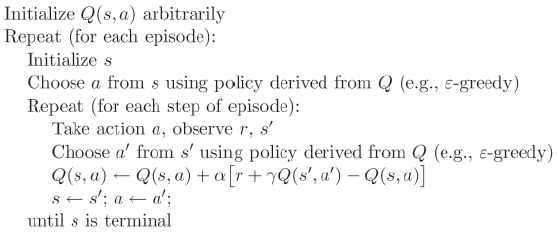
\includegraphics[width=0.8\textwidth]{Bilder/Sarsa.png}
	\caption{Sarsa: On Policy TD Control Algorithmus}
	\label{fig:Sarsa}
\end{figure}


\subsection{Off-Policy: Q-Learning}
Auch das Q-Learning Verfahren setzt auf den Q-Werten auf und berechnet diese über die unten genannte Formel, die Teil des Algorithmus in Abbildung \ref{fig:QLearning} ist.

\begin{equation}
Q(s_{t},a_{t}) \leftarrow Q(s_{t},a_{t}) + \alpha [r_{t+1} + \gamma max_{a} Q(s_{t+1},a) - Q(s_{t},a_{t})]
\end{equation} 

Der Unterschied zum Sarsa-Algorithmus ist hierbei der Teil $\gamma max_{a} Q(s_{t+1},a)$. Anstelle den erwarteten Return $Q(s_{t+1},a_{t+1})$ für die gewählte Aktion $a'$ im Zustand $s'$ mit dem Discount-Faktor $\gamma$ zu multiplizieren wie es beim Sarsa-Algorithmus gemacht wird, wird hier diejenige Aktion bestimmt, die den größten Reward verspricht und deren Reward $max_{a} Q(s_{t+1},a)$ mit dem Discount-Faktor multipliziert. \textbf{Damit wird der Q-Wert $Q(s,a)$ unabhängig von der Strategie, allein auf Basis des Returns und der Q-Werte benachbarter Zustände aktualisiert!}. 
Unhabhängig davon, welche Aktion die $\epsilon$-Greedy Policy wählt, wird immer der Q-Wert zur Berechnung genommen, die den höchsten Reward verspricht und nicht der, des durch die Policy gewählten Nachbarn. 

\begin{figure}[htbp]
	\centering	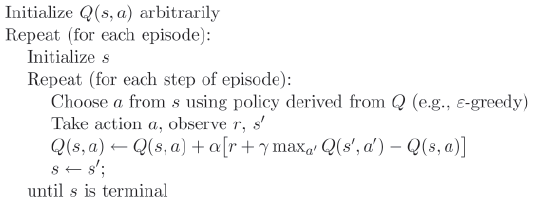
\includegraphics[width=0.8\textwidth]{Bilder/Q-Learning.png}
	\caption{Q Learning: Off Policy TD Control Algorithmus}
	\label{fig:QLearning}
\end{figure}


\subsection{Verhalten bei kleinem $\epsilon$}
Das Verhalten vom Sarsa-Algorithmus nähert sich dem vom Q-Learning an, da mit kleiner werdendem $\epsilon$ die Wahrscheinlichkeit sinkt eine zufällige Aktion auszuwählen. Bei sehr kleinem $\epsilon$ wird vermehrt die Aktion $a'$ ausgewählt, die den größten Reward verspricht, ähnlich wie es beim Q-Learning mit $max_{a} Q(s_{t+1},a)$ getan wird. Damit nährt sich das Verhalten von Sarsa dem des Q-Learnings an.

\section{Fragestellung 3: kontinuierliche Zustandsvariablen}
Für den Fall, dass die Zustandsvariablen kontinuierlich sind werden sie diskretisiert. Sollte der Zustandsraum durch die Diskretisierung zu groß werden, findet entweder eine Partitionierung des Zustandsraumes oder eine Abstraktion von Zuständen statt. Das heißt ein großer Zustandsraum kann in mehrere kleine Räume aufgeteilt werden, oder es wird über die Zustände selbst abstrahiert, d.h. mehrere Zustände werden zu einem zusammengefasst.

Ein Beispiel für die Partitionierung des Zustandsraumes ist Schach, bei dem der Zustandsraum in Eröffnung, Mittel- und Endspiel unterteilt werden kann. Ein Beispiel für die Abstraktion ist Kniffel, in dem bspw. die Sortierung der Würfel ignoriert wird um den Zustandsraum zu verkleinern. In diesem Fall werden dadurch nicht einmal Informationen verloren.

\subsection{Generalisierung durch überwachte Lernverfahren}

\todo{Nachfolgendes stammt aus dem Ertel}
Dadurch, dass es endlos viele Zustände gibt, wird auch die Tabelle gespeicherter Q- oder V-Werte unendlich groß. Hier gibt es die Möglichkeit, Methoden des überwachten Lernens zu verwenden, um die Werte zu generalisieren. Die Tabelle kann durch ein neuronales Netz ersetzt werden, welches als Input die Variablen $a$ und $s$ erhält und als Ziel-Output den Q-Wert besitzt. Für jede Aktualisierung des Q-Werts gibt es ein Trainingsbeispiel mit genannten Inputs und Outputs. Durch das neuronale Netz kann die Funktion $Q(s,a)$, welche für unendlich viele Eingaben definiert ist, auf einen endlichen Raum reduziert werden.
Statt eines neuronalen Netzes ist es auch möglich, andere überwachte Lernverfahren, wie beispielsweise Support Vector Machines zu verwenden, um den unendlichen Zustandsraum zu generalisieren und somit zu begrenzen.

Es kann aber Probleme geben, da der Q-Wert eigentlich erst nach unendlich vielen Besuchen der Zustands-Aktions-Paare zu seinem optimalen Wert konvergiert. Ein unendlich häufiger Besuch ist hier nicht mehr möglich, dementsprechend ist auch die Konvergenz nicht mehr garantiert gegeben.


\section{Fragestellung 4: Kniffel}
Dynamische Programmierung scheidet auf Grund des fehlenden Modells und der großen Zustandsmenge aus.

Q-Learning würde erst am Ende bewerten, bei Kniffel ist es aber wichtig die Zwischenschritte zu kennen?

Monte Carlo speichert bereits bewertete Paare und erlaubt daher die Bewertung jeden Schrittes. Ist aber speicheraufwendig.
Auf Grund der Problembeschaffenheit müssen alle Verfahren zusätzlichen Aufwand betreiben, um den Zustandsraum klein zu bekommen.

\todo{siehe den Link}
\url{http://www.haw-hamburg.de/fileadmin/user_upload/SchulCampus/Downloads/Arbeitskreis_Informatik/Kniffel_Agenten.pdf}
\listoftodos

\end{document}

